\documentclass{article}\usepackage[]{graphicx}\usepackage[]{color}
%% maxwidth is the original width if it is less than linewidth
%% otherwise use linewidth (to make sure the graphics do not exceed the margin)
\makeatletter
\def\maxwidth{ %
  \ifdim\Gin@nat@width>\linewidth
    \linewidth
  \else
    \Gin@nat@width
  \fi
}
\makeatother

\definecolor{fgcolor}{rgb}{0.345, 0.345, 0.345}
\newcommand{\hlnum}[1]{\textcolor[rgb]{0.686,0.059,0.569}{#1}}%
\newcommand{\hlstr}[1]{\textcolor[rgb]{0.192,0.494,0.8}{#1}}%
\newcommand{\hlcom}[1]{\textcolor[rgb]{0.678,0.584,0.686}{\textit{#1}}}%
\newcommand{\hlopt}[1]{\textcolor[rgb]{0,0,0}{#1}}%
\newcommand{\hlstd}[1]{\textcolor[rgb]{0.345,0.345,0.345}{#1}}%
\newcommand{\hlkwa}[1]{\textcolor[rgb]{0.161,0.373,0.58}{\textbf{#1}}}%
\newcommand{\hlkwb}[1]{\textcolor[rgb]{0.69,0.353,0.396}{#1}}%
\newcommand{\hlkwc}[1]{\textcolor[rgb]{0.333,0.667,0.333}{#1}}%
\newcommand{\hlkwd}[1]{\textcolor[rgb]{0.737,0.353,0.396}{\textbf{#1}}}%

\usepackage{framed}
\makeatletter
\newenvironment{kframe}{%
 \def\at@end@of@kframe{}%
 \ifinner\ifhmode%
  \def\at@end@of@kframe{\end{minipage}}%
  \begin{minipage}{\columnwidth}%
 \fi\fi%
 \def\FrameCommand##1{\hskip\@totalleftmargin \hskip-\fboxsep
 \colorbox{shadecolor}{##1}\hskip-\fboxsep
     % There is no \\@totalrightmargin, so:
     \hskip-\linewidth \hskip-\@totalleftmargin \hskip\columnwidth}%
 \MakeFramed {\advance\hsize-\width
   \@totalleftmargin\z@ \linewidth\hsize
   \@setminipage}}%
 {\par\unskip\endMakeFramed%
 \at@end@of@kframe}
\makeatother

\definecolor{shadecolor}{rgb}{.97, .97, .97}
\definecolor{messagecolor}{rgb}{0, 0, 0}
\definecolor{warningcolor}{rgb}{1, 0, 1}
\definecolor{errorcolor}{rgb}{1, 0, 0}
\newenvironment{knitrout}{}{} % an empty environment to be redefined in TeX

\usepackage{alltt}
\usepackage{geometry}
\usepackage{amsmath}
\usepackage{lscape}
\geometry{verbose,tmargin=2.5cm,bmargin=2.5cm,lmargin=2.5cm,rmargin=2.5cm}
\IfFileExists{upquote.sty}{\usepackage{upquote}}{}
\begin{document}



\begin{knitrout}
\definecolor{shadecolor}{rgb}{0.969, 0.969, 0.969}\color{fgcolor}\begin{kframe}
\begin{alltt}
\hlcom{# xy = matrix(runif(10000), ncol = 2) xy = xy[xy[,1] < 0.1 | xy[,2] < 0.1,]}
\hlcom{# xy = xy %*% matrix(c(1, 0.4, 0.4, 1), ncol = 2) xy = xy[xy[,1] <= 1 &}
\hlcom{# xy[,2] <= 1,]}

\hlstd{xyc} \hlkwb{=} \hlkwd{read.csv}\hlstd{(}\hlstr{"synthetic_data.csv"}\hlstd{)}
\hlstd{xy} \hlkwb{=} \hlstd{xyc[,} \hlnum{1}\hlopt{:}\hlnum{2}\hlstd{]}

\hlkwd{set.seed}\hlstd{(}\hlnum{1234}\hlstd{)}
\hlstd{subset} \hlkwb{=} \hlkwd{sample.int}\hlstd{(}\hlkwd{nrow}\hlstd{(xy),} \hlnum{300}\hlstd{)}

\hlkwd{library}\hlstd{(fastICA)}
\hlkwd{library}\hlstd{(NMF)}
\end{alltt}


{\ttfamily\noindent\itshape\color{messagecolor}{\#\# Loading required package: methods\\\#\# Loading required package: pkgmaker\\\#\# Loading required package: registry\\\#\# Loading required package: rngtools\\\#\# Loading required package: cluster\\\#\# NMF - BioConductor layer [OK] | Shared memory capabilities [OK] | Cores 7/8}}\begin{alltt}
\hlstd{fit.pca} \hlkwb{=} \hlkwd{prcomp}\hlstd{(xy,} \hlkwc{center} \hlstd{=} \hlnum{TRUE}\hlstd{,} \hlkwc{scale} \hlstd{=} \hlnum{FALSE}\hlstd{)}

\hlstd{temp} \hlkwb{=} \hlkwd{replicate}\hlstd{(}\hlnum{1000}\hlstd{,} \hlkwd{fastICA}\hlstd{(xy,} \hlnum{2}\hlstd{,} \hlkwc{method} \hlstd{=} \hlstr{"C"}\hlstd{),} \hlkwc{simplify} \hlstd{=} \hlnum{FALSE}\hlstd{)}
\hlstd{temp2} \hlkwb{=} \hlkwd{sapply}\hlstd{(temp,} \hlkwa{function}\hlstd{(}\hlkwc{x}\hlstd{)} \hlkwd{shapiro.test}\hlstd{(x}\hlopt{$}\hlstd{S)}\hlopt{$}\hlstd{statistic)}
\hlstd{fit.ica} \hlkwb{=} \hlstd{temp[[}\hlkwd{which.max}\hlstd{(temp2)]]}

\hlstd{fit.nmf} \hlkwb{=} \hlkwd{nmf}\hlstd{(}\hlkwd{t}\hlstd{(xy[subset, ]),} \hlkwc{rank} \hlstd{=} \hlnum{2}\hlstd{,} \hlkwc{nrun} \hlstd{=} \hlnum{20}\hlstd{,} \hlkwc{method} \hlstd{=} \hlstr{"snmf/r"}\hlstd{)}
\end{alltt}
\end{kframe}
\end{knitrout}

\begin{knitrout}
\definecolor{shadecolor}{rgb}{0.969, 0.969, 0.969}\color{fgcolor}\begin{kframe}
\begin{alltt}
\hlkwd{library}\hlstd{(NMF)}
\end{alltt}


{\ttfamily\noindent\itshape\color{messagecolor}{\#\# Loading required package: methods\\\#\# Loading required package: pkgmaker\\\#\# Loading required package: registry\\\#\# Loading required package: rngtools\\\#\# Loading required package: cluster\\\#\# NMF - BioConductor layer [OK] | Shared memory capabilities [OK] | Cores 7/8}}\begin{alltt}
\hlkwd{library}\hlstd{(RColorBrewer)}
\hlstd{pal} \hlkwb{=} \hlkwd{brewer.pal}\hlstd{(}\hlnum{3}\hlstd{,} \hlstr{"Set2"}\hlstd{)[}\hlkwd{c}\hlstd{(}\hlnum{2}\hlstd{,} \hlnum{3}\hlstd{,} \hlnum{1}\hlstd{)]}
\hlstd{pal} \hlkwb{=} \hlkwd{sapply}\hlstd{(pal,} \hlkwa{function}\hlstd{(}\hlkwc{col}\hlstd{)} \hlkwd{do.call}\hlstd{(rgb,} \hlkwd{c}\hlstd{(}\hlkwd{as.list}\hlstd{(}\hlkwd{col2rgb}\hlstd{(col)}\hlopt{/}\hlnum{255}\hlstd{),} \hlkwc{alpha} \hlstd{=} \hlnum{0.5}\hlstd{)))}
\hlstd{syms} \hlkwb{=} \hlkwd{c}\hlstd{(}\hlnum{19}\hlstd{,} \hlnum{4}\hlstd{,} \hlnum{21}\hlstd{)}
\hlstd{col} \hlkwb{=} \hlstd{pal[xyc[,} \hlnum{3}\hlstd{]]}
\hlstd{pch} \hlkwb{=} \hlstd{syms[xyc[,} \hlnum{3}\hlstd{]]}

\hlkwd{plot}\hlstd{(xy[subset,} \hlnum{1}\hlstd{], xy[subset,} \hlnum{2}\hlstd{],} \hlkwc{col} \hlstd{=} \hlstr{"black"}\hlstd{,} \hlkwc{pch} \hlstd{= pch[subset],} \hlkwc{xlab} \hlstd{=} \hlstr{"Gene 1"}\hlstd{,}
    \hlkwc{ylab} \hlstd{=} \hlstr{"Gene 2"}\hlstd{,} \hlkwc{xlim} \hlstd{=} \hlkwd{c}\hlstd{(}\hlnum{0}\hlstd{,} \hlnum{1}\hlstd{),} \hlkwc{ylim} \hlstd{=} \hlkwd{c}\hlstd{(}\hlnum{0}\hlstd{,} \hlnum{1}\hlstd{))}
\hlkwd{legend}\hlstd{(}\hlstr{"topright"}\hlstd{,} \hlkwc{legend} \hlstd{=} \hlkwd{c}\hlstd{(}\hlstr{"State A"}\hlstd{,} \hlstr{"State B"}\hlstd{,} \hlstr{"Transition State"}\hlstd{),} \hlkwc{pch} \hlstd{= syms[}\hlkwd{c}\hlstd{(}\hlnum{3}\hlstd{,}
    \hlnum{1}\hlstd{,} \hlnum{2}\hlstd{)],} \hlkwc{inset} \hlstd{=} \hlnum{0.05}\hlstd{)}
\end{alltt}
\end{kframe}

{\centering 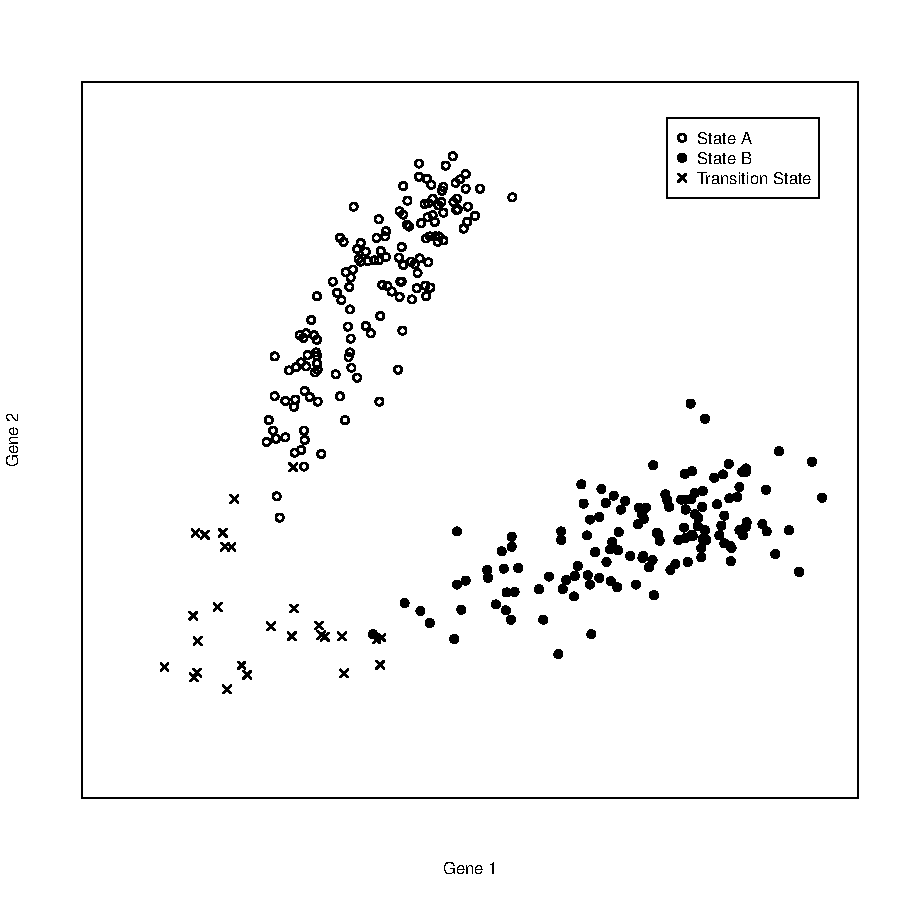
\includegraphics[width=\maxwidth]{figure/plots-1} 

}


\begin{kframe}\begin{alltt}
\hlkwd{plot}\hlstd{(xy[subset,} \hlnum{1}\hlstd{], xy[subset,} \hlnum{2}\hlstd{],} \hlkwc{col} \hlstd{=} \hlstr{"black"}\hlstd{,} \hlkwc{pch} \hlstd{= pch[subset],} \hlkwc{xlab} \hlstd{=} \hlstr{"Gene 1"}\hlstd{,}
    \hlkwc{ylab} \hlstd{=} \hlstr{"Gene 2"}\hlstd{,} \hlkwc{xlim} \hlstd{=} \hlkwd{c}\hlstd{(}\hlnum{0}\hlstd{,} \hlnum{1}\hlstd{),} \hlkwc{ylim} \hlstd{=} \hlkwd{c}\hlstd{(}\hlnum{0}\hlstd{,} \hlnum{1}\hlstd{))}
\hlcom{# legend('topright', legend = c('State A', 'State B', 'Transition State'),}
\hlcom{# pch = syms[c(3, 1, 2)], inset = 0.05)}
\hlkwd{legend}\hlstd{(}\hlstr{"topright"}\hlstd{,} \hlkwc{legend} \hlstd{=} \hlkwd{c}\hlstd{(}\hlstr{"PCA"}\hlstd{,} \hlstr{"ICA"}\hlstd{,} \hlstr{"NMF"}\hlstd{),} \hlkwc{lty} \hlstd{=} \hlstr{"solid"}\hlstd{,} \hlkwc{lwd} \hlstd{=} \hlnum{5}\hlstd{,}
    \hlkwc{col} \hlstd{= pal,} \hlkwc{inset} \hlstd{=} \hlnum{0.05}\hlstd{)}
\hlkwd{arrows}\hlstd{(}\hlkwc{x0} \hlstd{=} \hlkwd{rep}\hlstd{(}\hlkwd{mean}\hlstd{(xy[,} \hlnum{1}\hlstd{],} \hlnum{2}\hlstd{)),} \hlkwc{y0} \hlstd{=} \hlkwd{rep}\hlstd{(}\hlkwd{mean}\hlstd{(xy[,} \hlnum{2}\hlstd{],} \hlnum{2}\hlstd{)),} \hlkwc{x1} \hlstd{= fit.pca}\hlopt{$}\hlstd{rotation[}\hlnum{1}\hlstd{,}
    \hlstd{]} \hlopt{+} \hlkwd{mean}\hlstd{(xy[,} \hlnum{1}\hlstd{]),} \hlkwc{y1} \hlstd{= fit.pca}\hlopt{$}\hlstd{rotation[}\hlnum{2}\hlstd{, ]} \hlopt{+} \hlkwd{mean}\hlstd{(xy[,} \hlnum{2}\hlstd{]),} \hlkwc{col} \hlstd{= pal[}\hlnum{1}\hlstd{],}
    \hlkwc{lwd} \hlstd{=} \hlnum{5}\hlstd{)}
\hlkwd{arrows}\hlstd{(}\hlkwc{x0} \hlstd{=} \hlkwd{rep}\hlstd{(}\hlkwd{mean}\hlstd{(xy[,} \hlnum{1}\hlstd{],} \hlnum{2}\hlstd{)),} \hlkwc{y0} \hlstd{=} \hlkwd{rep}\hlstd{(}\hlkwd{mean}\hlstd{(xy[,} \hlnum{2}\hlstd{],} \hlnum{2}\hlstd{)),} \hlkwc{x1} \hlstd{= fit.ica}\hlopt{$}\hlstd{A[}\hlnum{1}\hlstd{,}
    \hlstd{]} \hlopt{+} \hlkwd{mean}\hlstd{(xy[,} \hlnum{1}\hlstd{]),} \hlkwc{y1} \hlstd{= fit.ica}\hlopt{$}\hlstd{A[}\hlnum{2}\hlstd{, ]} \hlopt{+} \hlkwd{mean}\hlstd{(xy[,} \hlnum{2}\hlstd{]),} \hlkwc{col} \hlstd{= pal[}\hlnum{2}\hlstd{],} \hlkwc{lwd} \hlstd{=} \hlnum{5}\hlstd{)}
\hlkwd{arrows}\hlstd{(}\hlkwc{x0} \hlstd{=} \hlkwd{c}\hlstd{(}\hlnum{0}\hlstd{,} \hlnum{0}\hlstd{),} \hlkwc{y0} \hlstd{=} \hlkwd{c}\hlstd{(}\hlnum{0}\hlstd{,} \hlnum{0}\hlstd{),} \hlkwc{x1} \hlstd{=} \hlkwd{basis}\hlstd{(fit.nmf)[}\hlnum{1}\hlstd{, ],} \hlkwc{y1} \hlstd{=} \hlkwd{basis}\hlstd{(fit.nmf)[}\hlnum{2}\hlstd{,}
    \hlstd{],} \hlkwc{col} \hlstd{= pal[}\hlnum{3}\hlstd{],} \hlkwc{lwd} \hlstd{=} \hlnum{5}\hlstd{)}
\end{alltt}
\end{kframe}

{\centering 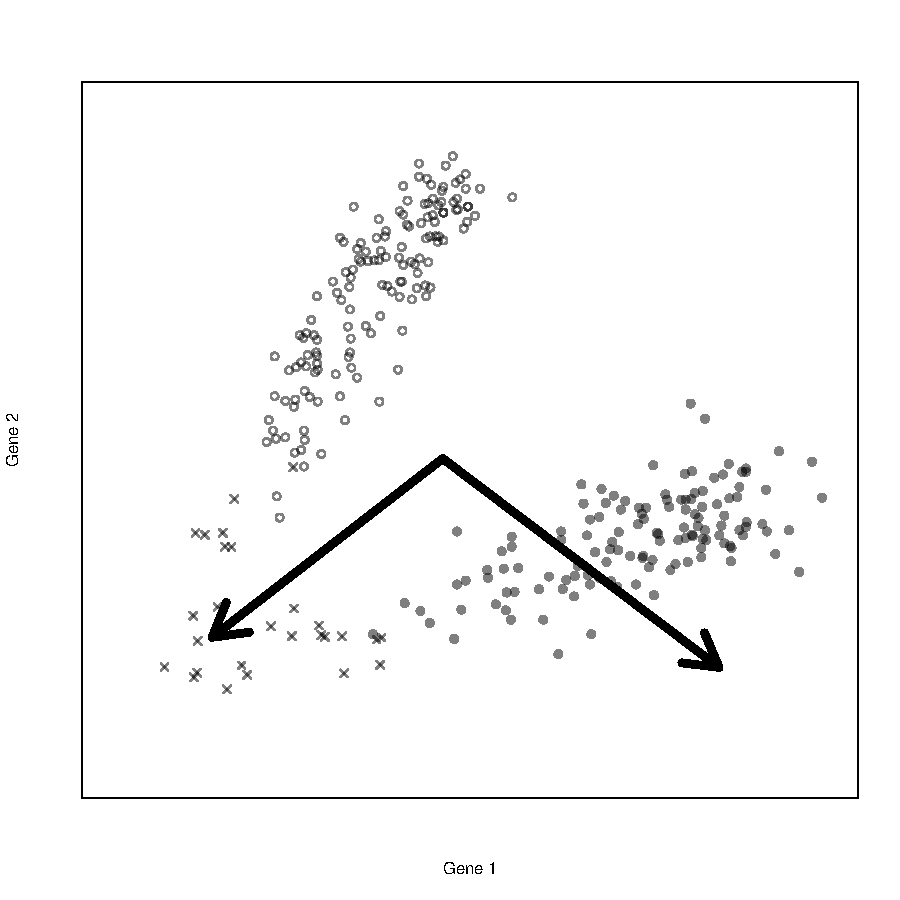
\includegraphics[width=\maxwidth]{figure/plots-2} 

}


\begin{kframe}\begin{alltt}
\hlkwd{plot}\hlstd{(fit.pca}\hlopt{$}\hlstd{x[subset, ],} \hlkwc{pch} \hlstd{= pch[subset],} \hlkwc{xlab} \hlstd{=} \hlstr{"PC1"}\hlstd{,} \hlkwc{ylab} \hlstd{=} \hlstr{"PC2"}\hlstd{,} \hlkwc{main} \hlstd{=} \hlstr{"PCA Projection"}\hlstd{)}
\end{alltt}
\end{kframe}

{\centering 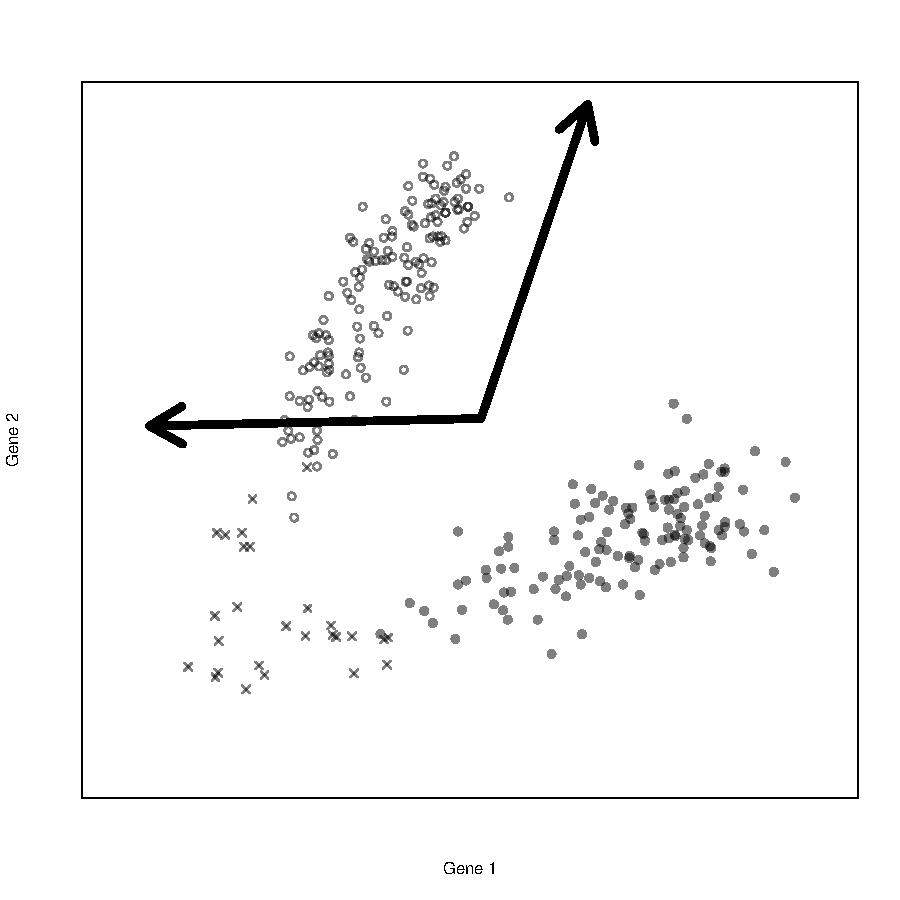
\includegraphics[width=\maxwidth]{figure/plots-3} 

}


\begin{kframe}\begin{alltt}
\hlkwd{plot}\hlstd{(fit.ica}\hlopt{$}\hlstd{S[subset, ],} \hlkwc{pch} \hlstd{= pch[subset],} \hlkwc{xlab} \hlstd{=} \hlstr{"C1"}\hlstd{,} \hlkwc{ylab} \hlstd{=} \hlstr{"C2"}\hlstd{,} \hlkwc{main} \hlstd{=} \hlstr{"ICA Projection"}\hlstd{)}
\end{alltt}
\end{kframe}

{\centering 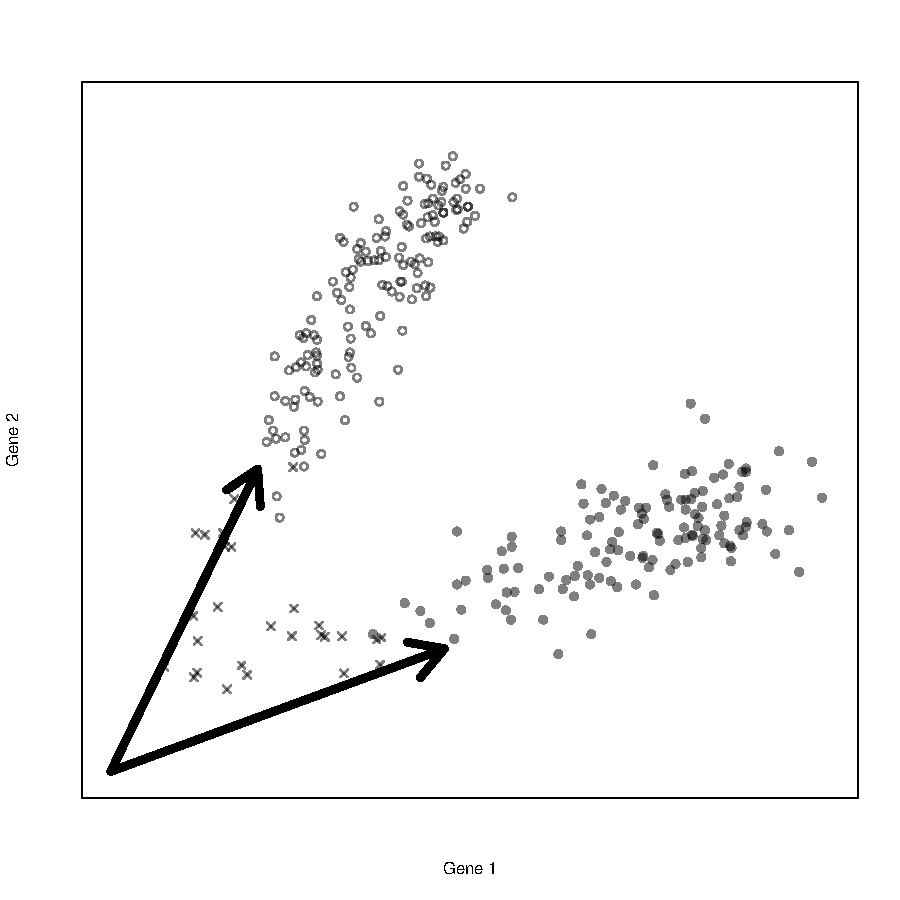
\includegraphics[width=\maxwidth]{figure/plots-4} 

}


\begin{kframe}\begin{alltt}
\hlkwd{plot}\hlstd{(}\hlkwd{t}\hlstd{(}\hlkwd{coef}\hlstd{(fit.nmf)),} \hlkwc{pch} \hlstd{= pch[subset],} \hlkwc{xlab} \hlstd{=} \hlstr{"F1"}\hlstd{,} \hlkwc{ylab} \hlstd{=} \hlstr{"F2"}\hlstd{,} \hlkwc{main} \hlstd{=} \hlstr{"NMF Projection"}\hlstd{)}
\end{alltt}
\end{kframe}

{\centering 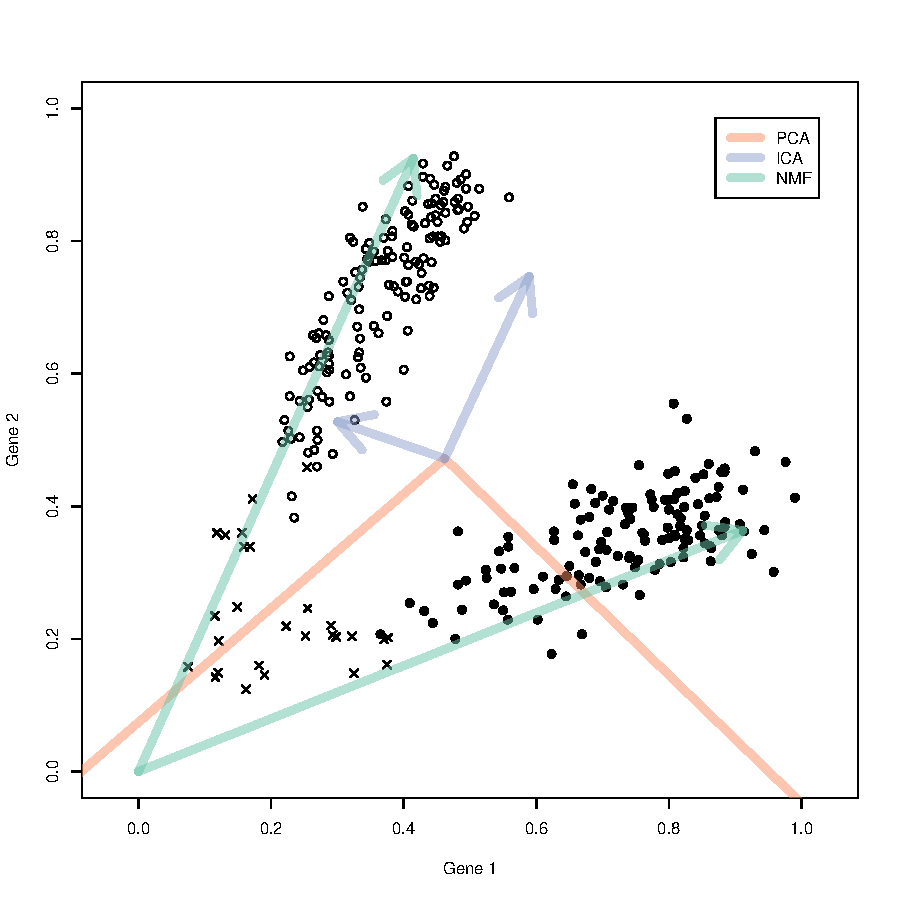
\includegraphics[width=\maxwidth]{figure/plots-5} 

}



\end{knitrout}

\end{document}
